\documentclass[11pt]{article}

\usepackage{geometry}
\geometry{
  a4paper,
  total={170mm,257mm},
  left=20mm,
  top=20mm,
}

\usepackage{amsmath}
\usepackage{hyperref}
\usepackage{url}
\usepackage{graphicx}
\usepackage{siunitx}
\usepackage{natbib}
\usepackage{siunitx}

\newcommand{\figplaceholder}[2]{%
  \begin{figure}[ht]
  \centering
  \fbox{\rule{0pt}{2.4in}\rule{0.9\linewidth}{0pt}}
  \caption{#2}
  \label{#1}
  \end{figure}
}

\title{Plume-Traj: Backward Source Attribution and Forward Dispersion}
\author{Alexander Ukhov, Ibrahim Hoteit}
\date{KAUST, December 2025}

\begin{document}
\maketitle

\section*{Introduction}

In atmospheric science, particularly in the study of volcanic eruptions, determining the source parameters of an airborne plume is a critical task. The height and timing of emissions of materials such as sulfur dioxide (SO$_2$) and ash are key inputs to atmospheric transport models used to forecast the plume's trajectory and potential impacts on aviation, air quality, and climate. However, direct measurements of these emission parameters during an eruption or after are often difficult or impossible to obtain. %In turn, satellite instruments can detect volcanic plumes and provide the total column density of volcanic material (e.g., SO$_2$).

In modeling, volcanic emissions can be prescribed using time-dependent vertical profiles. A widely used approach to derive vertical emission profiles for volcanic plume prediction is to perform trial-and-error adjustments, comparing satellite-based total column observations of the plume with model simulations that assume different emission heights. Inverse modeling methods are considered a more efficient and versatile approach for obtaining optimal emissions than the trial-and-error method. 

Here, we introduce an intermediate method implemented in the developed \texttt{Plume-Traj} tool for reconstructing volcanic emissions, using backward-in-time parcel trajectories and enabling the inference of time-dependent altitudes of volcanic material. The \texttt{Plume-Traj} can be used when the satellite measurement captures the enhanced values of SO$_2$, aerosol Index (AI), or Aerosol Optical Depth (AOD). Volcanic eruption monitoring relies on both source attribution (when and how high the material was injected) and also on forward dispersion (where the material travels after release). Therefore, we also offer a tool for the forward dispersion of volcanic material.


\section{Methodology}
These two instruments require precomputed dimensional meteorological fields computed using the Weather Research and Forecasting (WRF-Chem) model \citep{skamarock2005description,grell2005fully}, which has been recently corrected and updated in terms of simulating the volcanic eruptions \citep{ukhov2025enhancing}

\begin{itemize}
  \item \textbf{Backward source attribution:} \texttt{plume\_backtraj.py} starts from a satellite-retrieved column and traces a large number of virtual air parcels backward in time to a receptor vicinity, which is prescribed using a cylinder spanning the whole atmospheric column. By identifying the time and altitude at which these back-trajectories intersect with a cylinder, the script provides an estimate of the time-height profile of emission information.
  \item \textbf{Forward dispersion:} \texttt{plume\_forwtraj.py} releases a vertical column of parcels at the source and advects them forward to map transport pathways and parcel ages.
\end{itemize}
Optional physics includes gravitational settling of ash and sulfate aerosols, and SO$_2$ mass correction with prescribed e-folding lifetime.



\subsection{Input Data}
Both workflows of the \texttt{Plume-Traj} require meteorological data: one or more WRF \texttt{wrfout} files containing grid geometry (\path{XLAT}, \path{XLONG}, \path{DX}, \path{DY}, map factors), winds (\path{U}, \path{V}, \path{W}), geopotential (\path{PH}, \path{PHB}), and \path{Times}. When multiple files are supplied, they are assumed to be ordered in time (or provided via a sortable wildcard).
   


\subsection{Parcel Initialization for backward-in-time run}
The backward-in-time simulation begins at a specified time (parameter \path{--start-time}) by defining the starting locations of the backward-in-time trajectories. This is achieved through a process called parcel seeding:
\begin{itemize}
    \item The location of the volcanic plume is defined by satellite-derived data, typically provided as a NetCDF file. This file contains a 2D field representing the total vertical column density of some substance (e.g., SO$_2$ column, AI, or AOD) on the same horizontal grid as the WRF data. A plume mask is created from the satellite column data (\texttt{--column-var}) (optionally scaled by \path{--column-coef})  by identifying all grid cells where the substance's concentration exceeds a user-defined threshold (\texttt{--threshold}). Within this masked area, a specified number (\texttt{--n-columns}) of horizontal locations is randomly chosen.
    \item At each of these locations, a vertical line of parcels (\texttt{--n-vert}) is initialized, distributed randomly between a minimum (\texttt{--z-min}) and maximum (\texttt{--z-max}) altitude. Parcels are placed in the corresponding WRF grid cell.
    \item Parcels can also be released from columns randomly sampled inside the defined region \path{--seed-bbox}.
\end{itemize}
%This process generates thousands of virtual air parcels that collectively represent the observed plume structure at the simulation's start time. 




\subsection{Parcel Initialization for forward-in-time run}
Forward runs require a source location or a seed box:
\begin{itemize}
  \item \path{--source-lat}, \path{--source-lon} for a single column, or \path{--seed-bbox} with \path{--n-columns} for random source columns.
  \item Parcels are initialized between \path{--z-min} and \path{--z-max} with \path{--n-vert} samples. The run spans \path{--start-time} to \path{--end-time}.  
\end{itemize}



\subsection{Backward/forward Trajectory Calculation}
The core of both scripts is the backward/forward advection of air parcels. The position of each parcel is integrated backward/forward in time using a fourth-order Runge-Kutta (RK4) numerical scheme.
\begin{equation}
    \frac{d\vec{x}}{dt} = \vec{v}(\vec{x}, t)
\end{equation}
For the backward mode, the integration is performed as:
\begin{equation}
    \vec{x}(t - \Delta t) \approx \vec{x}(t) - \vec{v}(\vec{x}, t) \Delta t
\end{equation}
The velocity vector $\vec{v}$ for each parcel is determined by interpolating the U, V, and W wind components from the surrounding WRF grid points in both space and time. The parameter \path{--integration-dt}, in seconds, controls the advection time step. Each parcel carries a weight derived from the column field, enabling both count-based and mass-weighted diagnostics.

\subsection{Gravitational settling of aerosols}

For aerosol species, the tool can account for gravitational settling by incorporating a size-and altitude-dependent terminal velocity. In WRF-Chem, ash particles are categorized into 10 size bins based on their radii, ranging from 0.01955 to 1000.0 µm, see Table \ref{tab:particle_size_divided}. For ash gravitational settling, terminal velocities are calculated for the mean arithmetic radii ($R_{m}$) within each bin. Ash density is assumed to be 2500 \unit{kg\ m^{-3}}, sulfate density is 1800 \unit{kg\ m^{-3}}, and it is assumed that sulfate particles have a dry volume median radius = 0.62 $\mu$m. The lookup table (\texttt{misc/settling\_velocity\_data.py}) for different aerosol types (e.g., \texttt{vash\_1} through \texttt{vash\_10}, and \texttt{sulf}) is being used to apply an additional settling velocity to the parcels during advection. The lookup table values of settling velocity profiles were computed in \cite{ukhov2025enhancing}. For aerosol types (e.g. \texttt{sulf}, \texttt{vash\_1}\ - \texttt{vash\_{10}}) a settling velocity profile can be added using \path{--aer-type}.


\begin{table}[h!]
\centering
\begin{tabular}{|c|c|c|c|c|}
\hline
Bin & Radius lower bound (µm) & Radius upper bound (µm) & $R_\text{m}$ (µm) & Density (\unit{kg\ m^{-3}}) \\ \hline
vash\_1 & 500 & 1000 & 500 & 2500 \\
vash\_2 & 250 & 500 & 375 & 2500 \\
vash\_3 & 125 & 250 & 187.5 & 2500 \\
vash\_4 & 62.5 & 125 & 93.75 & 2500 \\
vash\_5 & 31.25 & 62.5 & 46.88 & 2500 \\
vash\_6 & 15.625 & 31.25 & 23.44 & 2500 \\
vash\_7 & 7.8125 & 15.625 & 11.72 & 2500 \\
vash\_8 & 3.90625 & 7.8125 & 5.86 & 2500 \\
vash\_9 & 1.95325 & 3.9065 & 2.93 & 2500 \\
vash\_{10} & 0.01955 & 1.95325 & 0.97 & 2500 \\ \hline
\end{tabular}
\caption{Ash particle bin size ranges with corresponding WRF-Chem ash bins.}
\label{tab:particle_size_divided}
\end{table}



\begin{figure}[h!]
    \centering
    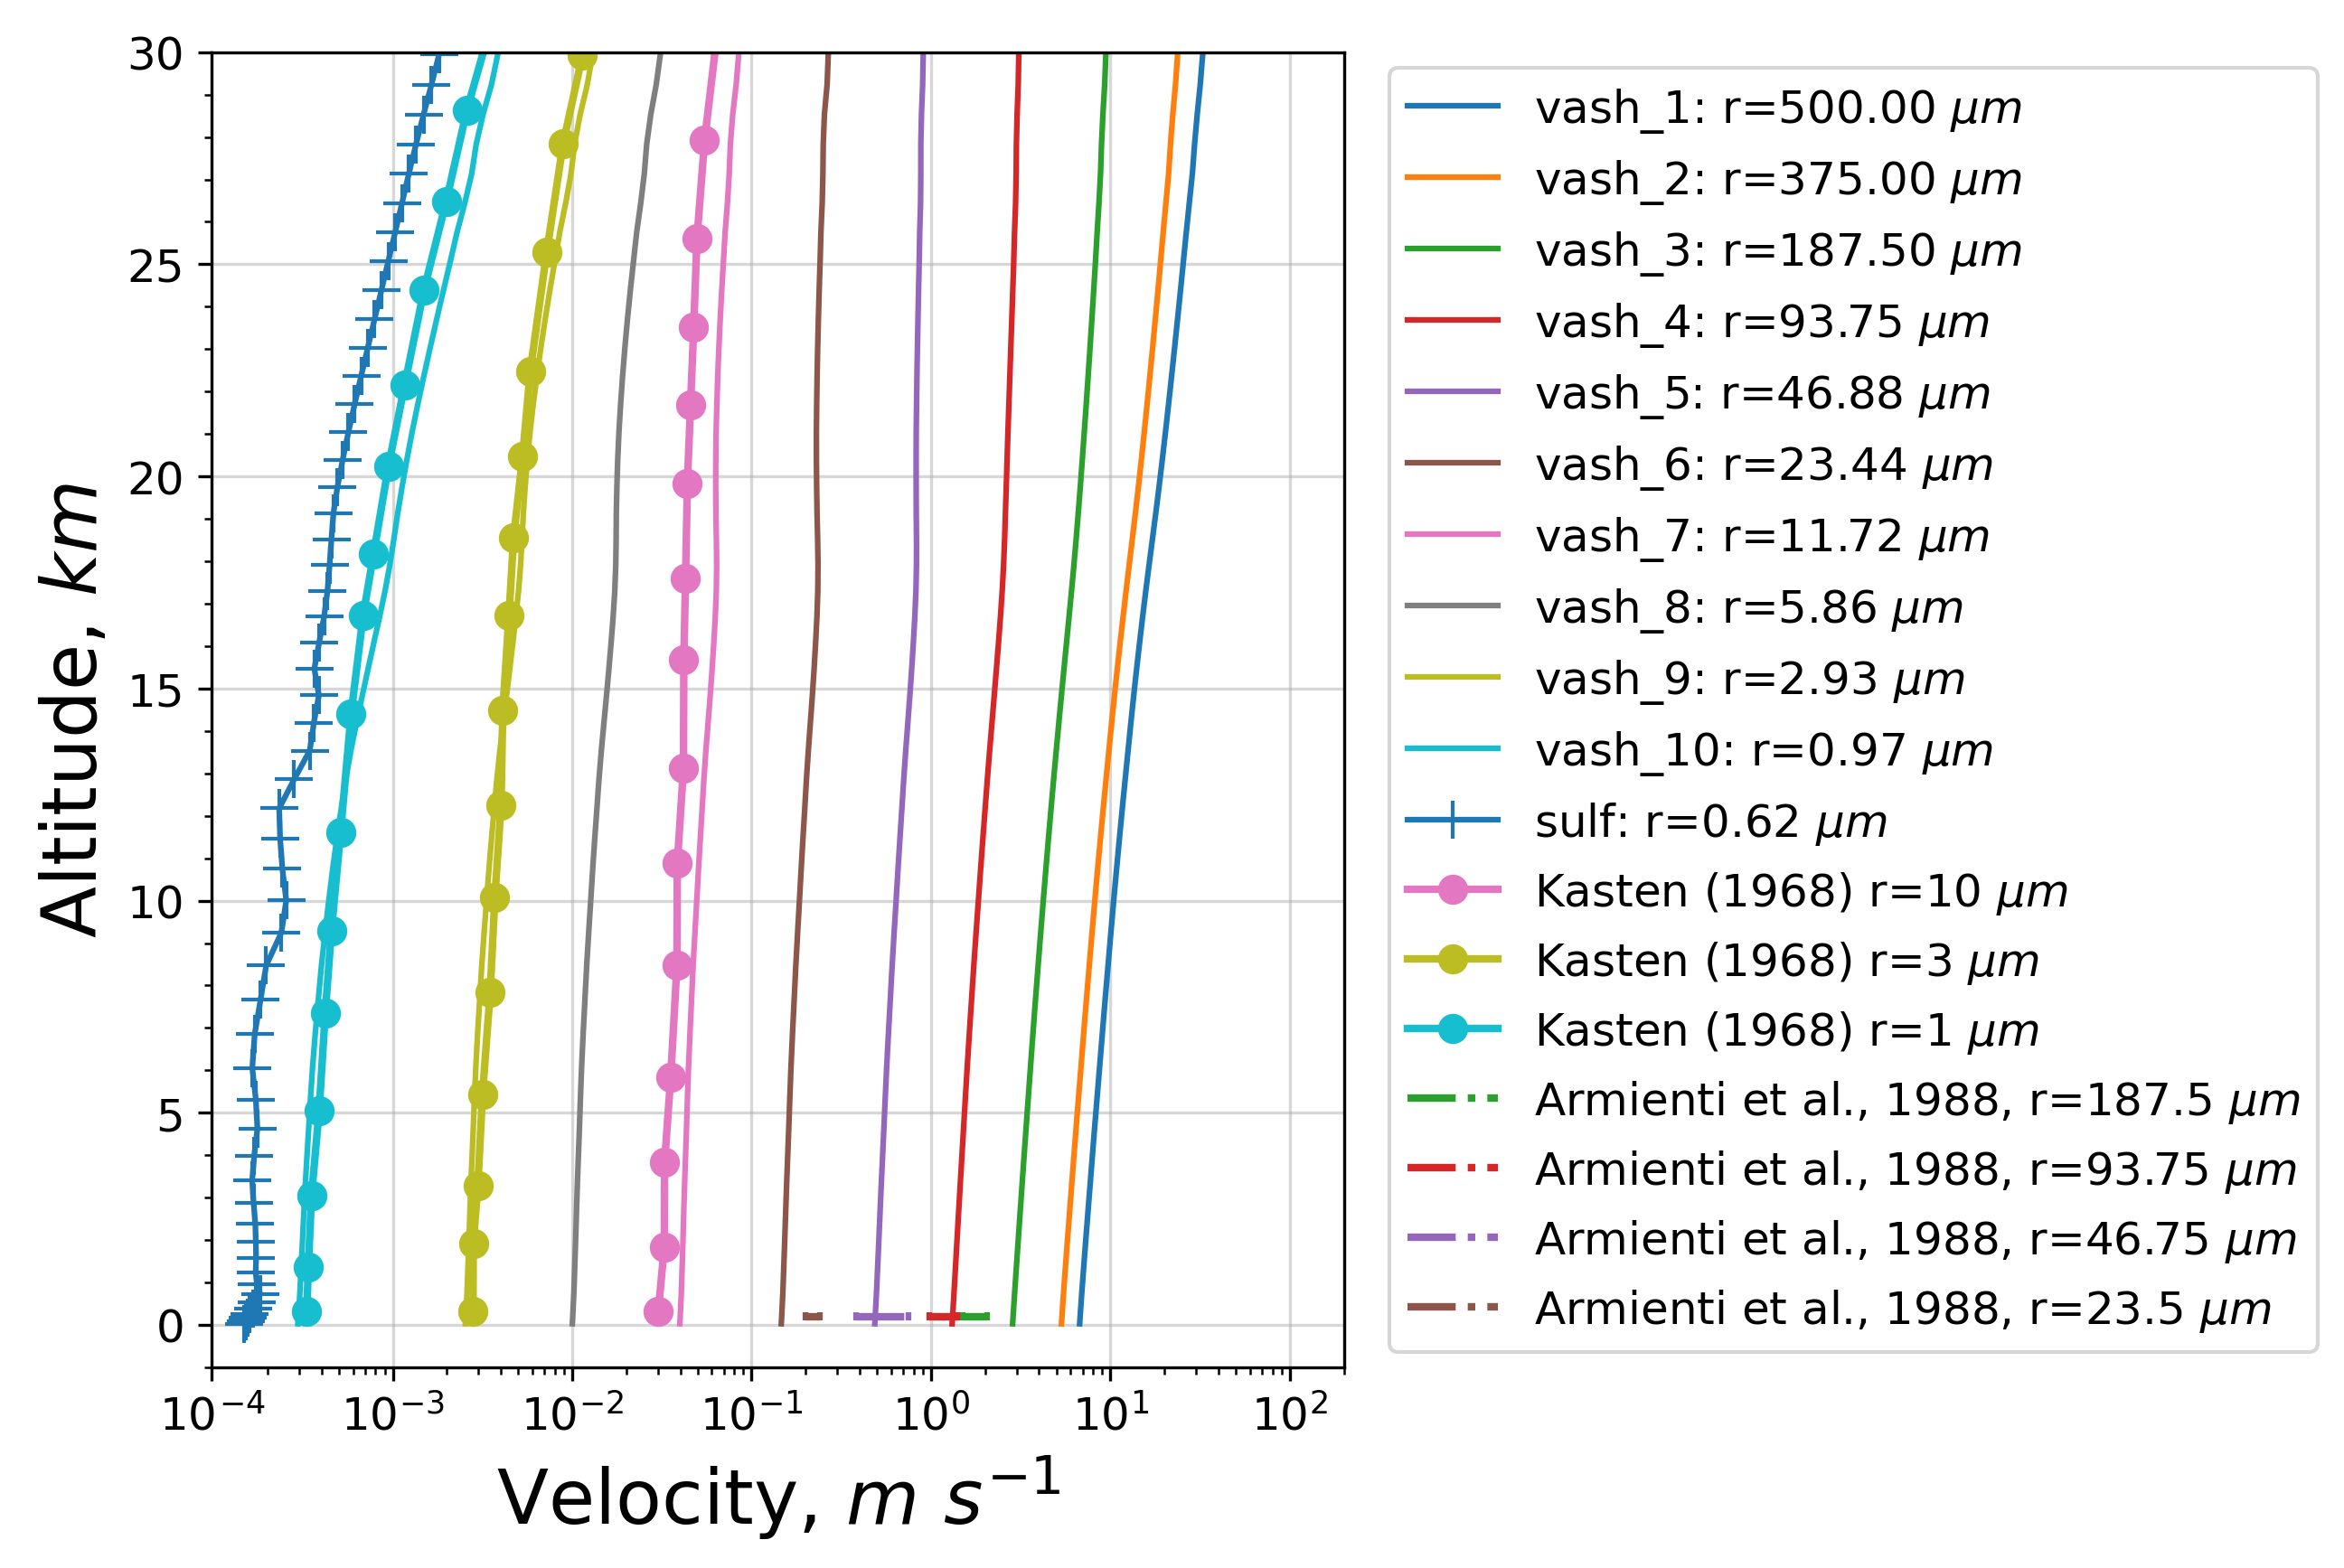
\includegraphics[width=0.8\linewidth]{./Fig1.png}
    \caption{Settling velocity as a function of altitude computed for ash
    particles with different radii and for sulfate particles with dry volume median
    radii = 0.62~$\mu$m. Comparison with theoretical data by
    \cite{kasten1968falling} and \cite{armienti1988numerical}.}
    \label{fig:grav_settl_velocities}
\end{figure}

Figure \ref{fig:grav_settl_velocities} illustrates the settling velocities of ash particles as a function of altitude for multiple particle radii. The gravitational settling velocity of sulfate particles having dry volume median radii = 0.62~$\mu$m is also shown. We compare our results with theoretical formulations by \cite{kasten1968falling} and \cite{armienti1988numerical}. In \cite{kasten1968falling}, settling velocities are for spherical particles with radii of 1~$\mu$m, 3~$\mu$m, and 10~$\mu$m; for comparison, the density of these particles was adjusted to align with that of ash. In \cite{armienti1988numerical}, ranges of terminal velocities are provided for feldspar mineral particles (radii of 23.5~$\mu$m, 46.75~$\mu$m, 93.75~$\mu$m, and 187.5~$\mu$m), which are regarded as having the closest density to ash particles.


\subsection{Source Attribution}
To identify the origin of the plume, a cylindrical "receptor" region is defined around the known coordinates of the source (\texttt{--receptor-lat}, \texttt{--receptor-lon}). This cylinder has a user-defined radius (\texttt{--receptor-radius}) and vertical extent (\texttt{--receptor-min-h}, \texttt{--receptor-max-h}). During the backward integration, the script continuously checks if a parcel has entered this receptor cylinder. If a parcel's trajectory intersects the cylinder, it is considered to have "arrived" at the receptor.  Parcel arrivals are binned on a time-height grid with \path{--arrival-bin-minutes}. If both \path{--emission-start} and \path{--emission-end} are supplied, fixed time bins spanning the emission window are used and arrivals outside the window are ignored. The simulation stops for a parcel if it leaves the model domain or reaches the beginning of the emission window (\texttt{--emission-start}).
\\
Mass-weighted outputs use the column value multiplied by cell area and divided by \path{--n-vert}. If \path{--so2-efolding-days} is set, parcel masses are adjusted backward in time using an exponential correction to compensate for SO$_2$ oxidation (or radioactive decay, for example).


\section{Output}
All input parameters and output results can be serialized and stored in a pickle file using \path{--state-pickle}. The file includes grid data, trajectories, emission matrices, and metadata, allowing plots to be reproduced without re-running the solver. \texttt{plot\_backtraj.py} and \texttt{plot\_forwtraj.py} regenerate the same plots from a saved \path{--state-pickle} file. The aggregation scripts in \texttt{misc/aggregate\_backtraj.py} and \texttt{misc/aggregate\_forwtraj.py} combine multiple pickles and output the aggregated plots, for example, for \texttt{vash\_1}\ - \texttt{vash\_{10}} parcels. All plotting commands accept \path{--map-extent} to override map bounds when needed and may also include a vertical seed distribution plot (\path{--seeds-vertical-figure}). \\

For demonstration purposes the tool was deployed in both modes for the Hayli Gubbi eruption on 23 November 2025. We the backward in time run we use observations of $_2$ and the aerosol index from TROPOMI on 24 November at 11:00 UTC. These examples are implemented in the code \url{https://github.com/saneku/Plume-traj} by default.

\subsection{Output from the backward in time run}
The script \texttt{plume\_backtraj.py} generates a series of quantitative and visual outputs, see Fig. \ref{fig:fig2}.


\begin{itemize}
    \item Emission Time-Height Matrix (\texttt{--output-txt}, \texttt{--output-figure}): The primary output is a 2D histogram that bins the "arrived" parcels by their arrival time and altitude. This matrix, saved as both a text file and a plot, represents the estimated emission profile from the source, showing the most likely periods and altitudes of significant emissions.

    \item Trajectory Plots (\texttt{--trajectory-figure}): A map showing the horizontal paths of all parcels that successfully reached the receptor. Trajectories are colored by an attribute, such as their initial altitude, providing a visual link between the observed plume and the source.

    \item Diagnostic Plots: Several other figures are generated for detailed analysis:
    \begin{itemize}
        \item \texttt{--seeds-figure}: A map of the initial horizontal positions of the seeded parcels, overlaid on the satellite column data.
        \item \texttt{--missed-trajectory-figure}: A map showing the trajectories of parcels that did \emph{not} reach the receptor, which can be useful for diagnosing the influence of the wind field.
        \item \texttt{--trajectory-age}: A plot of trajectories colored by the time taken to travel from the plume to the source.
        \item \texttt{--trajectory-arrival-height-figure}: Trajectories colored by the height at which they arrived at the receptor.
    \end{itemize}    
\end{itemize}


\begin{figure}[h!]
    \centering
    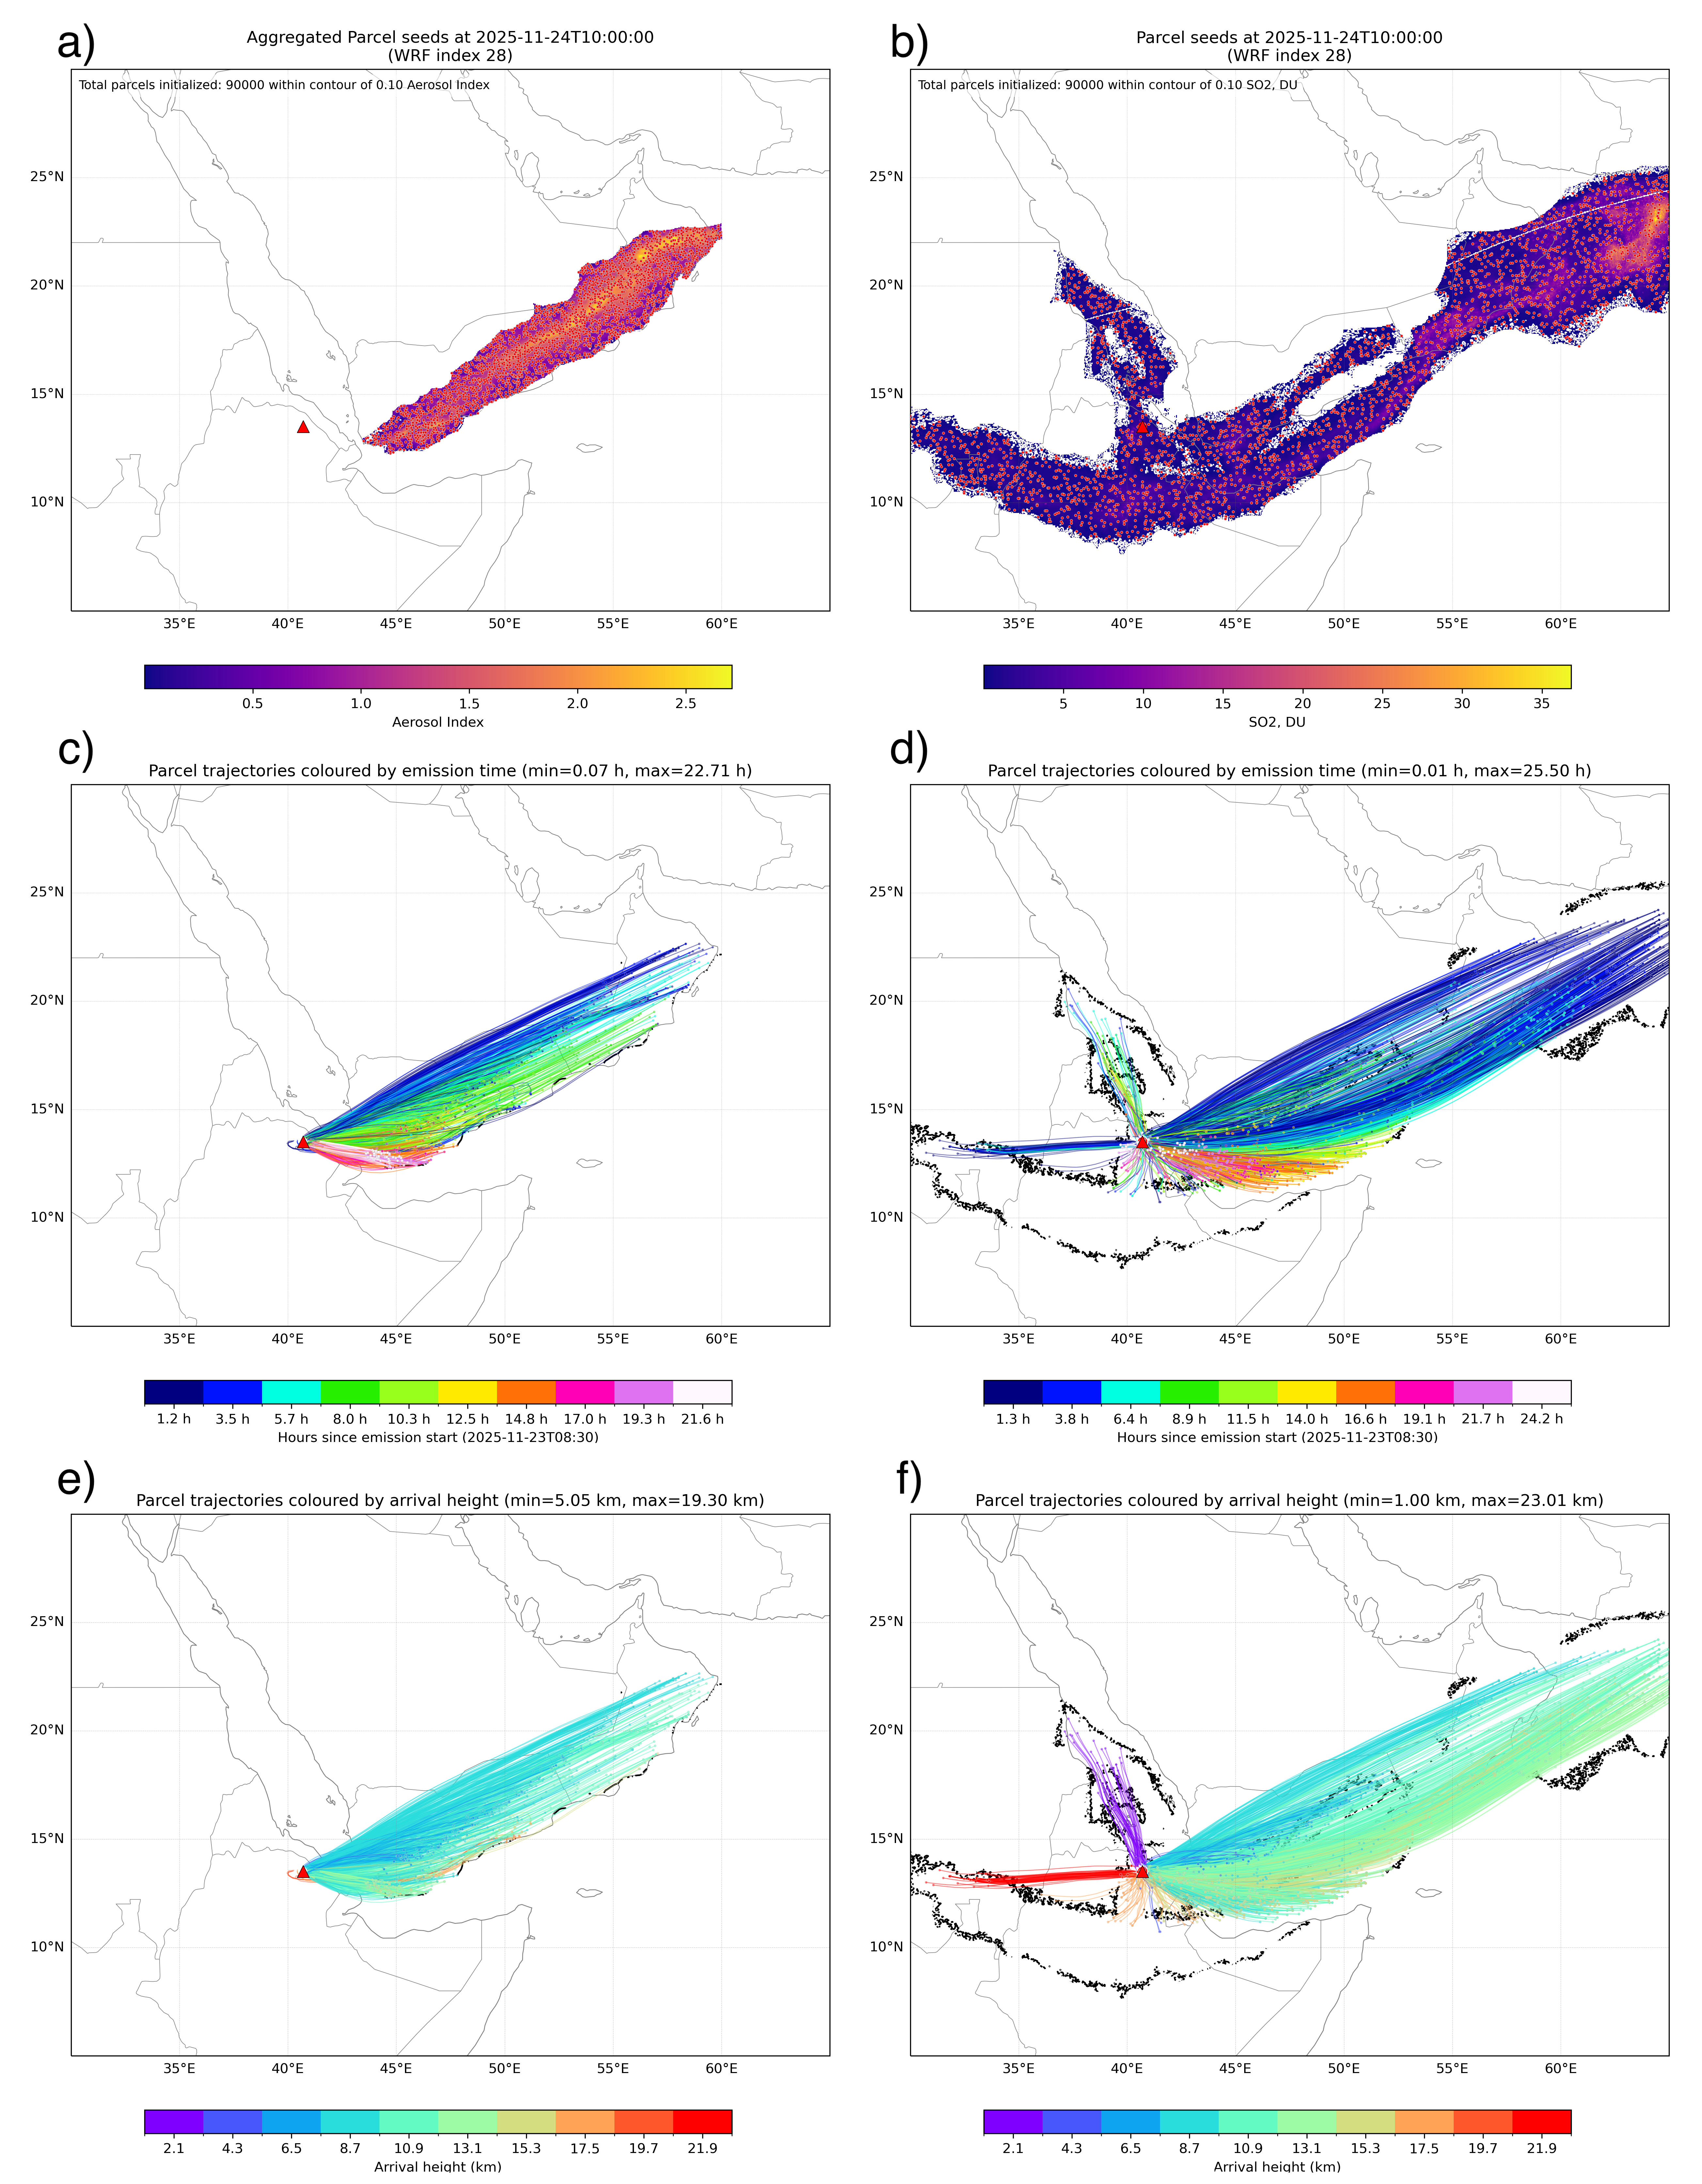
\includegraphics[width=1.0\linewidth]{Fig2.png}
    \caption{Backward‐trajectory reconstruction of the volcanic source using the \textit{Plume-traj} tool (\url{https://github.com/saneku/Plume-traj}). Ash - left column, SO$_2$ - right column. Panels a) and b) show the spatial distribution of parcel "seeds" initialized within the TROPOMI-derived Aerosol Index (AI) a) and TROPOMI SO$_2$ column loading b) on 24 November 2025, at 11:00 UTC. Panels c) and d) show backward parcel trajectories, shaded according to the number of hours elapsed since the start of the emission, thereby indicating the distribution of arrival times at the site of the Hayli Gubbi volcano. Panels e) and f) show the corresponding arrival heights. Threshold values for ash and SO$_2$ fields are 0.1 and highlighted by black contour lines. The red triangle marks the Hayli Gubbi volcano.}
    \label{fig:fig2}
\end{figure}

\clearpage

\subsection{Output from the forward in time run}
The script \texttt{plume\_forwtraj.py} is for forward runs and writes height-colored and age-colored trajectory maps (\path{--height-figure}, \path{--age-figure}), see Fig. \ref{fig:fig3}.

\begin{figure}[h!]
    \centering
    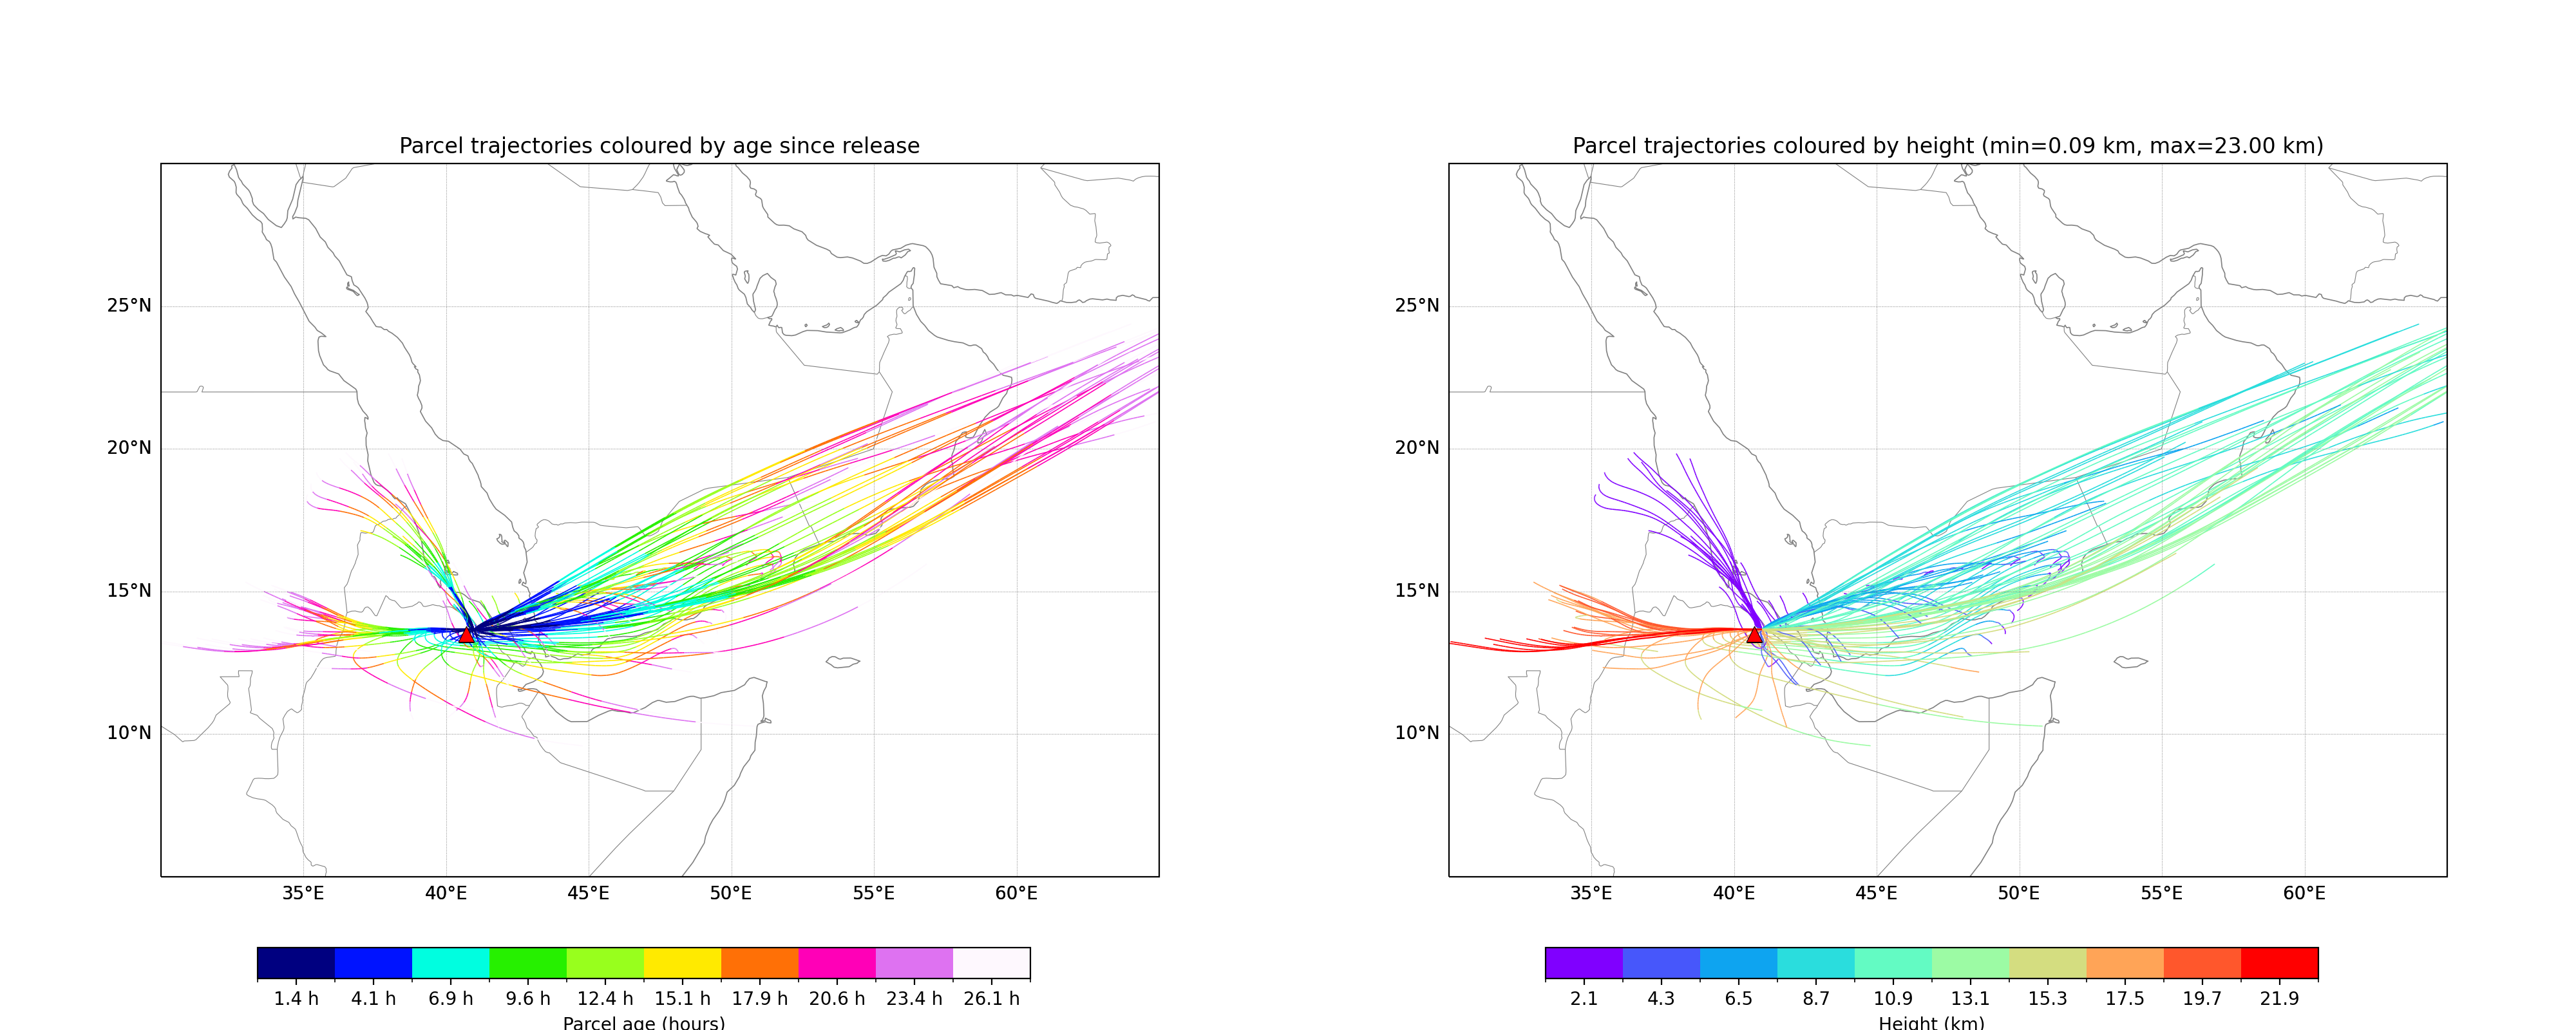
\includegraphics[width=0.90\linewidth]{Fig3.png}
    \caption{Aggregated forward trajectories for ash (vash\_6...vash\_{10}) colored by age (time since the release) (left) and height (right). Computed by forward in time mode using the \textit{Plume-traj} tool (\url{https://github.com/saneku/Plume-traj}.}
    \label{fig:fig3}
\end{figure}


\section{Coupling to \textit{PrepEmisSources}}
The emission matrices obtaned in backward in time mode provide a direct bridge to the emission scenarios used by \textit{PrepEmisSources} \citep{ukhov_2025_16856541}. This links observed plume retrievals to physically consistent emission scenarios that can be injected into WRF-Chem via \textit{PrepEmisSources}. A typical coupling workflow is:
\begin{enumerate}
\item Run \texttt{Plume-Traj} with \path{--emission-start} and \path{--emission-end} aligned to the WRF-Chem simulation window.
\item Use the computed mass-weighted matrix (\path{--mass-output-txt}) (see Fig. \ref{fig:Fig4}) as the time-height distribution of emitted mass; 
\item Normalize the matrix to match the desired total emitted SO$_2$ or ash mass and translate the matrix into the emission scenario format using the \textit{PrepEmisSources}, preserving the time bin edges and vertical structure, see Fig. \ref{fig:Fig5}.
\end{enumerate}


\begin{figure}[h]
    \centering
    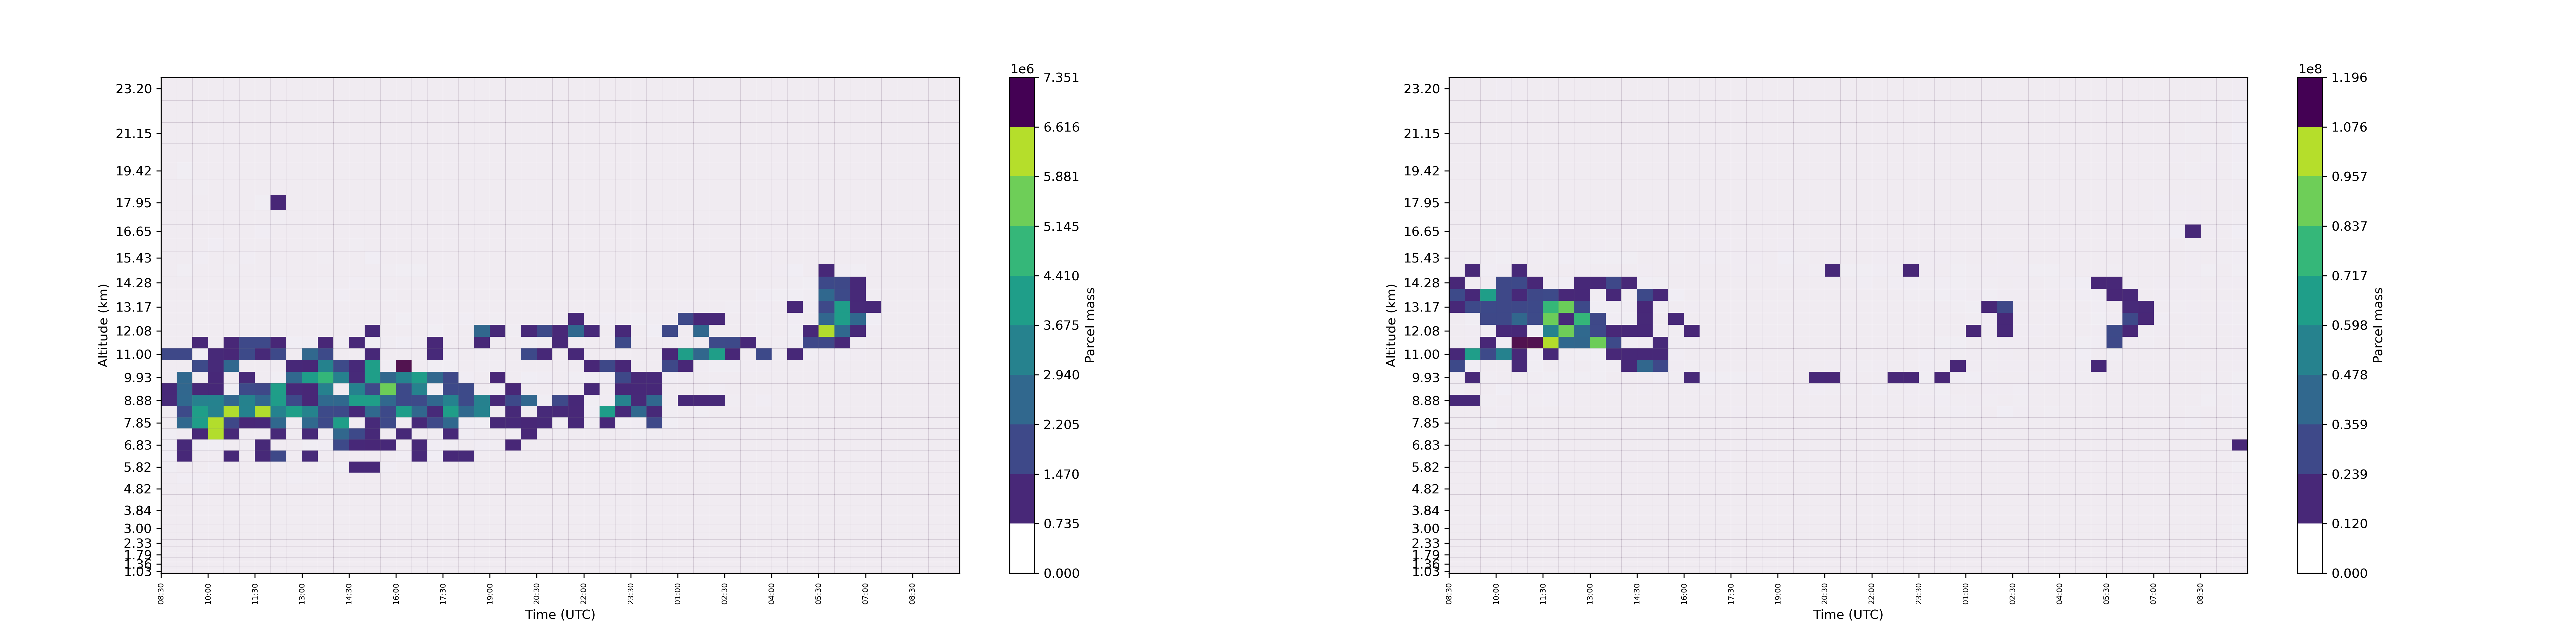
\includegraphics[width=1.0\linewidth]{Fig4.png}
    \caption{Reconstructed time-height emission matrix based on parcels' age and arrival height, see Fig. \ref{fig:fig2}, respectively. Aggregated ash age parcels (left), SO$_2$ parcels age (right). Parcels mass in arbitrary units.}
    \label{fig:Fig4}
\end{figure}

\begin{figure}[h]
    \centering
    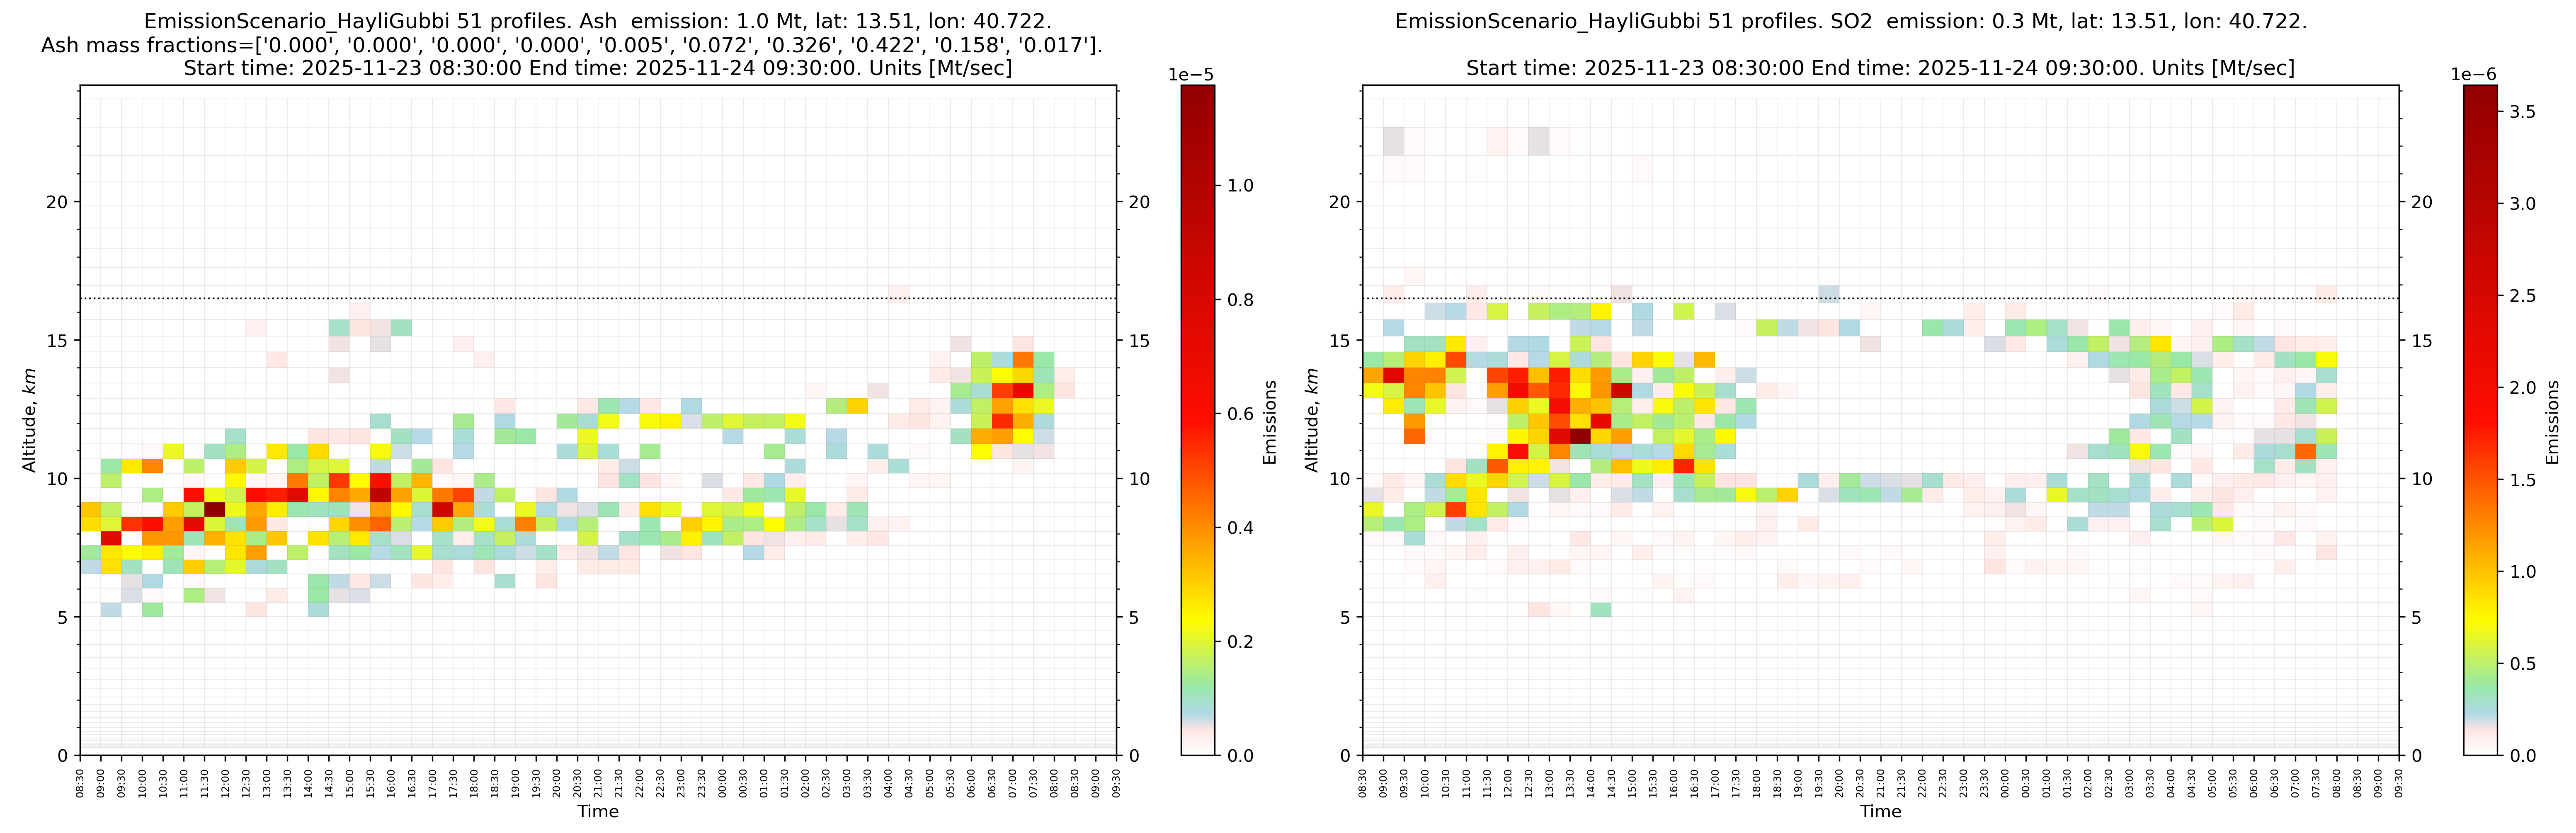
\includegraphics[width=1\linewidth]{Fig5.png}
    \caption{Normalised by erupted mass emission scenarios obtained for ash (left) and  SO$_2$ (right). Plots are constructed using the \textit{PrepEmisSources} utility \cite{ukhov_2025_16856541} }
    \label{fig:Fig5}
\end{figure}


\bibliographystyle{plainnat}
\bibliography{refs}

\end{document}
